\documentclass[times, utf8, zavrsni, numeric]{fer}
\usepackage{booktabs}
\usepackage{titlesec}
\newcommand{\sectionbreak}{\clearpage}
\frenchspacing
\begin{document}

\thesisnumber{5628}
\title{Web aplikacija za predstavljanje portfelja programera}
\author{Mislav Vuletić}
\maketitle
\zahvala{}
Posvećeno svima koji su voljni učiti i neprestano napredovati.
\tableofcontents

\chapter{Uvod}
\qquad Prilikom traženja posla prednost je ako se programer može predstaviti potencijalnom poslodavcu sa svim projektima u kojima je sudjelovao i programskom podrškom koju je razvio.
Često se za tu svrhu koriste LinkedIn\footnotemark{} ili Git\footnotemark{} stranice, odnosno druge vlastite web stranice programera.
Učinkovito predstavljanje može se postići uz pomoć jedne web stranice koja će omogućavati direktne poveznice na projekte do Git alata (sadržavati linkove na aktivne projekte) te omogućiti međusoban kontakt programera i poslodavca putem korisničkog sučelja.
\footnotetext{LinkedIn - poslovno orijentirana društvena mreža}
\footnotetext{Git - sustav za upravljanje izvornim kodom nastao 2005.~godine}

Ovaj rad opisuje kroz postupak dizajniranja i postavljanja aktivne web stranice programera.
Fokus rada nije na izradi najjednostavnijeg rješenja, već se želi postići skalabilno rješenje kojim se funkcionalnost stranice može proširiti u bilo kojem trenutku.

U drugom poglavlju predstavljeno je idejno rješenje, odnosno funkcionalni i nefunkcionalni zahtjevi te su ukratko navedeni slični projekti i postojeća zanimljiva rješenja.
U trećem poglavlju opisana je tehnologija korištena pri izradi web aplikacije. Četvrto poglavlje sadrži opis rješenja, odnosno tumačenje uporabe razvijene web aplikacije.
Naposljetku, zaključak sadrži rezime cijelog rada, odnosno komentar o tome je su li ispunjeni svi funkcionalni i nefunkcionalni zahtjevi te se ukratko navode sve direktne poveznice na kojima se nalazi sadržaj web aplikacije.

\chapter{Ideja}
\section{Funkcionalni i nefunkcionalni zahtjevi}
\qquad Vlastita portfolio web stranica programera mora sadržavati opće informacije o programeru, u prvom redu informacije za kontakt te direktne poveznice na stranice Git repozitorija i stranice društvenih mreža.
Programsko rješenje mora omogućavati komunikaciju s programerom direktno na stranici, poput slanja mail poruka.
Nadalje, web stranica mora imati dobro strukturirani odjeljak za prikaz projekata na kojima je programer radio.
To znači da svaki projekt mora imati svoje mjesto na stranici koje će sadržavati naziv projekta, kratki opis projekta, sliku projekta te mogući daljnji sadržaj prema potrebi.
Na stranici mora postojati način za pregledavanje CV dokumenta, odnosno životopisa u pdf formatu.

Portfolio web stranica programera mora koristiti vlastitu domenu programera.
Mora biti podignuta na udaljenom poslužitelju.
Stranica mora biti moderna i jednostavna.
Drugim riječima mora biti privlačna potencijalnom poslodavcu.
Web sjedište također mora biti jednostavno i intuitivno za korištenje, što podrazumijeva direktne poveznice za laku navigaciju.

\section{Portfolio stranice nekih programera}
\qquad Prije početka dizajniranja vlastitih portfolio stranica cilj je bio istražiti kako su drugi programeri postigli učinak privlačenja pažnje potencijalnih poslodavaca.
Stranica \textit{www.creative-portfolios.com} nam je uvelike olakšala posao s obzirom na to da se održava dnevno te se mogu pratiti promjene na stranicama GitHub-a.
Web sjedišta koja se posebno ističu su: \textit{cihadturhan.com}, \textit{fishnation.de} te \textit{eli.wtf}.
Ono što ove stranice čini vrijednima je autentičnost te vrlo intuitivno pronalaženje informacija.
Slika 2.1 prikazuje stranicu \textit{cihadturhan.com} na kojoj se vrlo pregledno uočavaju trenutne vještine programera.
Na slici 2.2 možemo vidjeti prikaz projekata na stranici \textit{fishnation.de}.
Na slici 2.3 se nalazi stranica s dobro strukturiranim općim informacijama o programeru sa stranice \textit{eli.wtf/about}.

\begin{figure}[htb]
				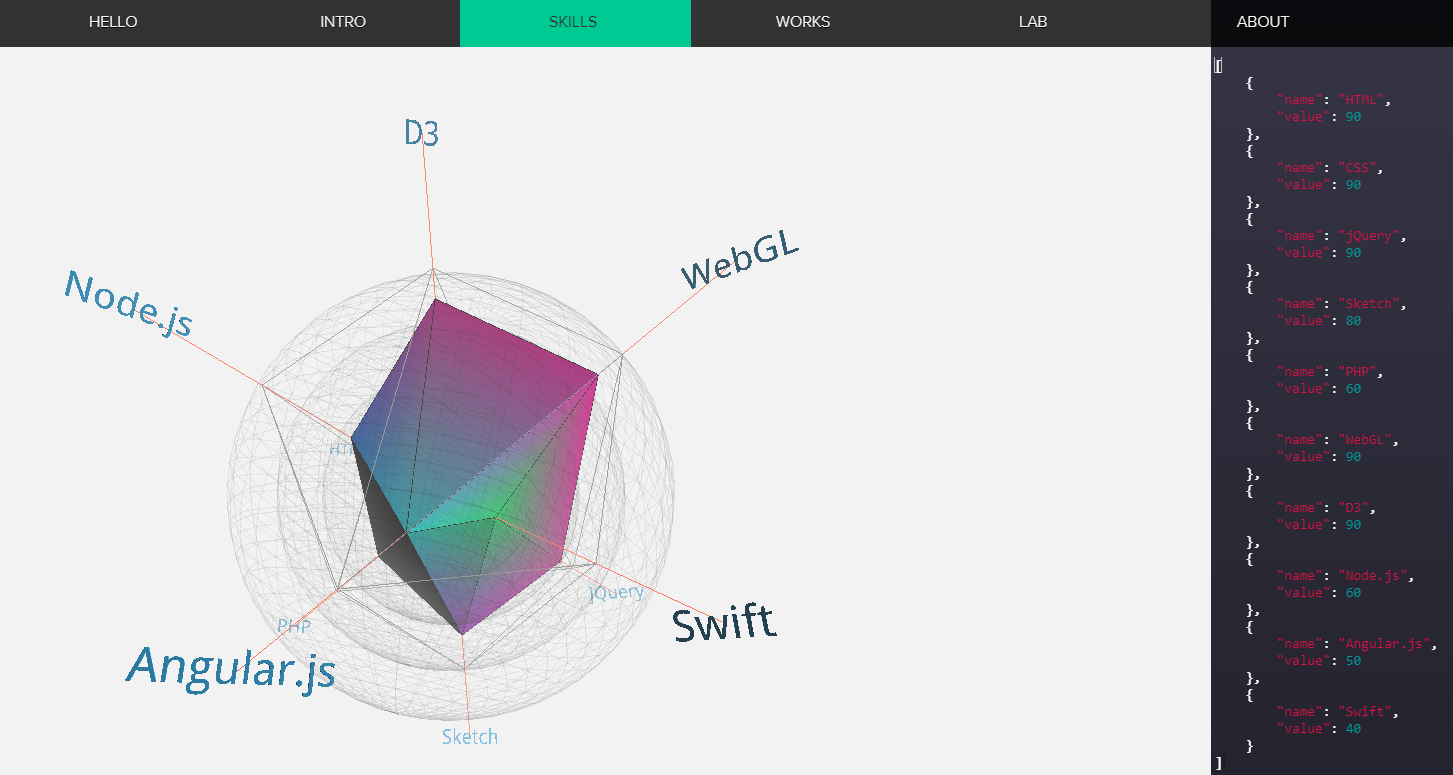
\includegraphics[width=14.6cm]{images/skills.png}
				\caption{Prikaz vještina programera}
				\label{fig:skills}
\end{figure}

\begin{figure}[htb]
				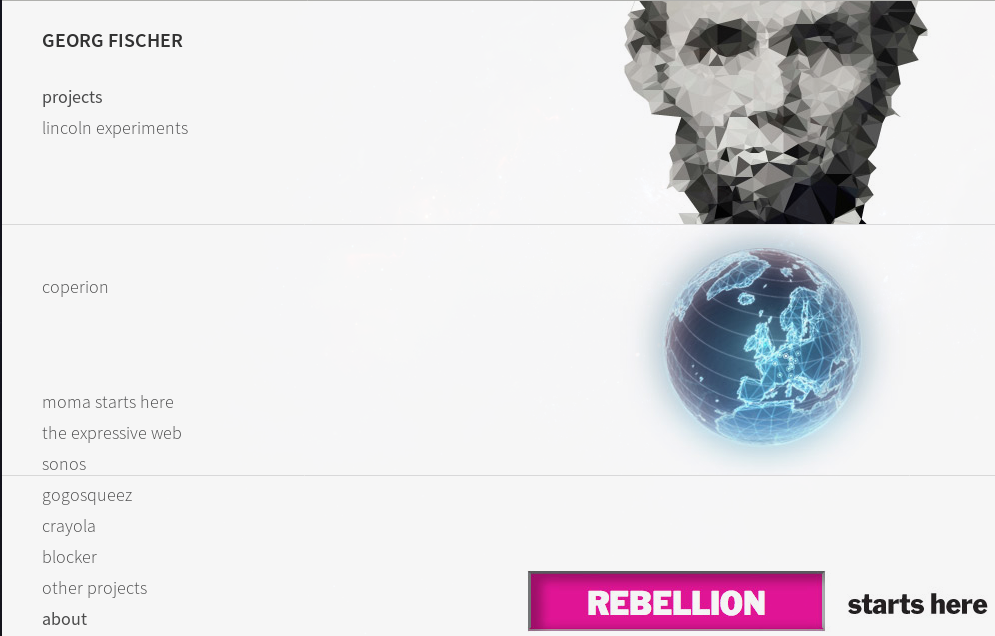
\includegraphics[width=14.6cm]{images/fishnation.png}
				\caption{Prikaz projekata programera}
				\label{fig:fishnation}
\end{figure}

\begin{figure}[htb]
				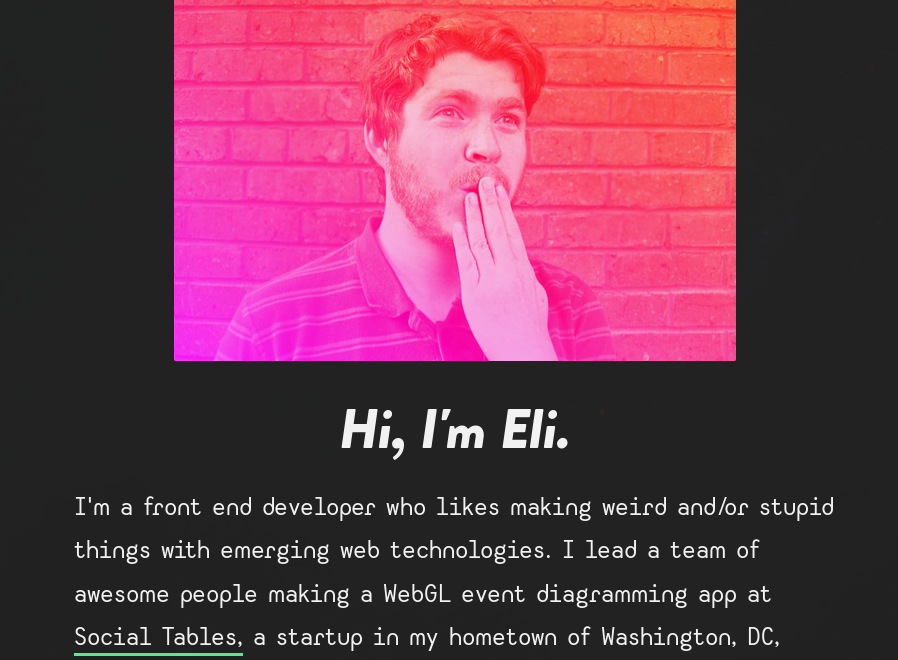
\includegraphics[width=14.6cm]{images/eli.png}
				\caption{Prikaz općih informacija o programeru}
				\label{fig:eli}
\end{figure}

\chapter{Korištene tehnologije}
\section{Jezik i generiranje pogleda}
\subsection{Programski jezik Java}
\qquad Java je objektno orijentirani programski jezik razvijen iz programskoj jezika Oak\footnotemark{}.
\footnotetext{Oak - programski jezik razvijen 1991., evoluirao u programski jezik Java 1995.}
Glavna ideja u razvoju programskog jezika Java bila je potpora za višeplatformnost.
Tako se danas Javin virtualni stroj može izvoditi na gotovo svim platformama; od Linuxa, Solarisa, Mac OS-a do Windowsa.
Druga bitna stavka je da je Java programerima potpuno nebitno hoće li se njihov program izvoditi na 32-bitnom ili 64-bitnom sustavu.
To je zato što Javina specifikacija definira apstraktni računski virtualni stroj kod kojeg je sve propisano.
\subsection{Thymeleaf}
\qquad Thymeleaf je suvremeni skup modela koji se koriste za razvitak samostojećih web aplikacija koje se izvode na poslužitelju.
Služi za izradu XHTML ili HTML5 datoteka.
Thymeleaf teži potpuno nadomjestiti \textit{JSP}\footnotemark{}, te učiniti tehnologiju jednostavnijom za korištenje.
\footnotetext{JSP - Java Server Pages, služi dinamičkom generiranju HTML, XML i drugih tipova datoteka}
Glavni razlog korištenja Thymeleaf-a jest što nudi elegantna rješenja za razvojni tijek rada kroz HTML.

\section{Java Spring Model-View-Controller}
\qquad Java Spring MVC je modul vrlo popularnog \textit{framework}-a Java Spring koji je zaživio u prvom desetljeću 21.~stoljeća.
Java Spring je \textit{open-source} biblioteka za Java platformu.
Omogućava lakši razvoj standardnih i \textit{enterprise}\footnotemark{} aplikacija.
\footnotetext{enterprise aplikacije - prevelika i prekompleksna aplikacija za individualno korištenje}
Java Spring MVC koristi popularnu strategiju izrada web stranica.
MVC definira tri cjeline koje su prikazane na slici 3.1; \textit{\textbf{M}odel} (model), \textit{\textbf{V}iew} (pogled), \textit{\textbf{C}ontroller} (upravitelj).

\begin{figure}[htb]
				\centering
				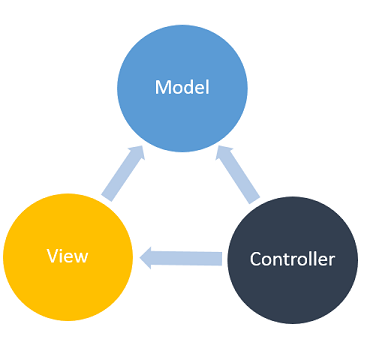
\includegraphics[width=5cm]{images/mvc.png}
				\caption{MVC struktura}
				\label{fig:mvc}
\end{figure}

\noindent
Ideja svake od tih cjelina je jasno odrediti gdje se koji dio aplikacije treba nalaziti.
\begin{itemize}
				\item Model uključuje \textit{backend}\footnotemark{}, te podatke aplikacije, odnosno poslovnu logiku i bazu podataka ako je aplikacija ima.
		\footnotetext{backend - pomoćni sustav, server}
	\item View (pogled) je dio koji korisnik naše aplikacije vidi; 
		html\footnote{html - Hyper Text Markup Language, prezentacijski jezik za izradu web stranica}, 
		css\footnote{css - Cascading Style Sheets, stilski jezik koji služi opisu html dokumenta}, 
		javascript\footnote{javascript - skriptni programski jezik koji se izvršava u web pregledniku}.
	\item Controller (upravitelj) upravlja korisničkim zahtjevima.
\end{itemize}
Dodatno Java Spring definira HandlerAdapter, HandlerInterceptor, HandlerMapping, LocaleResolver, MultipartResolver te ViewResolver koji definiraju gdje se dijelovi koda moraju nalaziti za lakše održavanje i razvitak EE\footnotemark{} aplikacija.
\footnotetext{EE - \textit{enterprise edition}, odnosno aplikacije velikog spektra}

\section{Pokretanje aplikacije na poslužitelju}
\subsection{Digital Ocean}
\qquad Digital Ocean je servis koji nudi najam poslužiteljskih računala na njihovom oblaku.
Usluga se naplaćuje.
Sjedište im je u New York-u, no imaju servere u cijelom svijetu što dopušta korisnicima da postave svoju aplikaciju na više lokacija po svijetu kako bi se njihova web stranica brže učitavala.
\subsection{Apache Tomcat}
\qquad Apache Tomcat program je \textit{open source} implementacija Javinih servleta te \textit{JSP} (Java Server Pages), \textit{JEL} (Java Expression Language) i \textit{JWS} (Java WebSocket) specifikacija razvijenih od Java programera.
Koristi se kao Web poslužitelj koji pruža potpuno Java okruženje na kojima se Java kod može izvoditi.
\subsection{Namecheap}
\qquad Namecheap je registar akreditiran od ICANN-a (krovne organizacije za upravljanje domenama).
Pruža usluge registracije domena te pretprodaje već registriranih domena.
Osim toga pruža i usluge najma računala poslužitelja.
Sjedište im je u Phoenixu, Arizona no nude usluge u cijelom svijetu.
Kompanija tvrdi da trenutno poslužuju sedam milijuna registriranih domena za otprilike tri milijuna klijenata.

\section{Korištene biblioteke}
\subsection{SimpleGrid.css}
\qquad Simple Grid je jednostavna css mreža koja omogućava dijeljenje stranice u 12 stupaca.
Prvenstveno je napravljena za primjenu na mobitelima. Svi se stupci protežu do rubova ekrana što je prednost na manjim ekranima.
U našem projektu ova biblioteka se koristi na stranici \textit{/projects} za jednostavniji razmještaj elemenata u web pregledniku.
\subsection{fullPage.js}
\qquad FullPage.js je tehnologija koja omogućava korisniku da vrlo jednostavno napravi web stranicu na kojoj je omogućeno pomicanje po stranici za po jednu visinu zaslona koristeći \textit{scroll} tipku\footnotemark{} na mišu.
\footnotetext{scroll - gumb klizača, nalazi se između lijeve i desne tipke na mišu}
Tehnologija je vrlo popularna te je koriste kompanije poput Google, Coca Cola, Ebay, itd.
\subsection{Google fonts}
\qquad Google fonts je kolekcija interaktivnih sučelja koja omogućuju korisniku odabir fonta za tekst koji se prikazuje na njegovoj stranici.
Usluga je podržana od strane kompanije Google te se ne naplaćuje niti sama usluga niti brzina dohvaćanja fonta s njihovih poslužiteljskih računala.
\subsection{CodePen api}
\qquad CodePen je socijalno mrežno okruženje za razvijanje jednostavnih programa koristeći \textit{html}, \textit{css} i \textit{javascript} direktno u web pregledniku.
Okruženje se sastoji od četiri polja, gdje tri od ta četiri pripadaju jezicima navedenima prije, a zadnje polje služi pregledu rezultata.
CodePen sučelje dozvoljava ugradnju tog okruženja u vlastitu stranicu.
\subsection{SvgBackgrounds}
\qquad SvgBackgrounds je priključak za web aplikacije.
Omogućava postavljanje \textit{SVG}\footnotemark{} pozadina veličine 5KB te je podržan od većine web preglednika koji se danas koriste.
\footnotetext{SVG - slike određene vektorima u XML formatu}

\chapter{Opis rješenja}
\qquad U sklopu ovog rada razvijeno je rješenje koje se sastoji od 7 Web stranica.
To je korijenska (početna) stranica koja se nalazi na poveznici \textit{mmedo.me} te ostalih 6 stranica koje se nalaze na stranicama \textit{/sayHi}, \textit{/about}, \textit{/resume}, \textit{/projects}, \textit{/resultMessage} te \textit{/error}.
Svaku od navedenih poveznica rješava pripadajući kontroler u Java Spring MVC poretku prosljeđujući pripadajući pogled.

\qquad U nastavku opisujemo svaku stranicu pojedinačno. Uz opis svake stranice također su priložene slike koje prikazuju izgled dotičnih stranica onako kako one izgledaju u vrijeme predaje završnog rada.
Slike su uslikane na web pregledniku FireFox 60.0 (64bit) na računalu s rezolucijom 1920x1080.
Bitno je naglasiti da je web stranica u potpunosti kompatibilna s modernim web preglednicima poput Google Chrome (verzija 66.0.x.x), Internet Explorer 8+, Opera 15+, itd.
Stranica također nudi potpunu podršku za web preglednike na modernim mobilnim uređajima koji dolaze s Androidom 4+, odnosno bilo kojim iPhone uređajem te web preglednicima za mobilne uređaje poput ranije navedenih Google Chrome, Mozilla Firefox, Opera te Safari.

\qquad Java Spring MVC aplikaciju pokreće Apache Tomcat na udaljenom poslužitelju u Frankfurtu.
Poslužiteljsko računalo je uzeto u najam putem usluge kompanije Digital Ocean za 5 dolara (32 kune) mjesečno.
To je najjeftinija opcija koju nude.
Razlog odabira dotične usluge jest što studenti imaju početnih 50 dolara pri izradi računa koje mogu potrošiti na usluge koje kompanija nudi.
Odabrani operacijski sustav je Ubuntu 16.4, izabran zbog jednostavnosti korištenja.
Adresa \textit{mmedo.me} je domena u najmu od kompanije Namecheap.
Konkretna domena košta 9 dolara (57 kuna) godišnje.
Projekt ukupno košta 440 kuna godišnje, odnosno 35 kuna mjesečno.

\pagebreak
\section{Početna stranica}
\qquad Početna stranica nalazi se na poveznici \textit{mmedo.me}. Na slici 4.1 možemo vidjeti izgled početne stranice.

\begin{figure}[htb]
				\centering
				
\includegraphics[width=14.6cm]{images/front-page.png}
				\caption{Izgled početne stranice}
				\label{fig:front-page}
\end{figure}

Na početnoj stranici se nalaze direktne poveznice za dolazak na ostale stranice; to je stranica koja omogućava slanje poruke programeru, stranica s informacijama o programeru, stranica projekata te brza poveznica za dohvaćanje životopisa programera.
Nadalje, na stranici se nalaze direktne poveznice do društvenih mreža programera (s lijeva na desno); Facebook, LinkedIn, YouTube, CodePen, GitHub, GitLab.

\begin{figure}[htb]
				\centering
				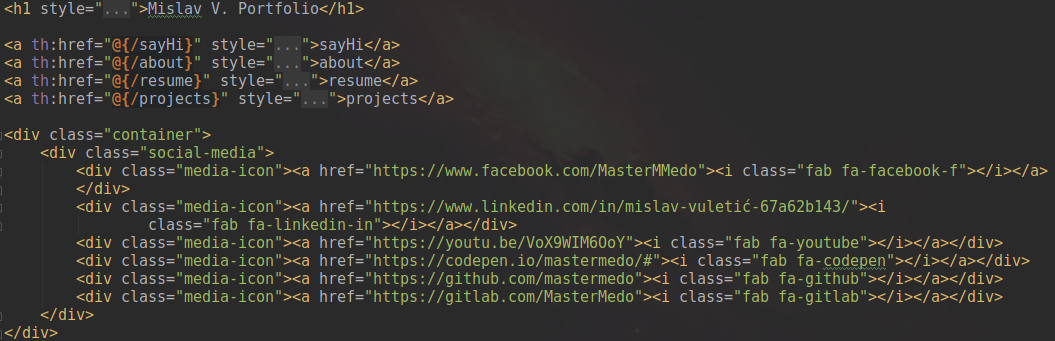
\includegraphics[width=14.6cm]{images/start-page.png}
				\caption{Kod početne stranice}
				\label{fig:start-page}
\end{figure}

\section{Stranica za slanje poruke}
\qquad Stranica za slanje poruke sadrži poveznicu za povratak na početnu stranicu te prostor za unos poruke i tipku za slanje poruke. Slika 4.3 prikazuje stranicu s primjerom poruke koji se nalazi na stranici pri učitavanju.

\begin{figure}[htb]
				\centering
				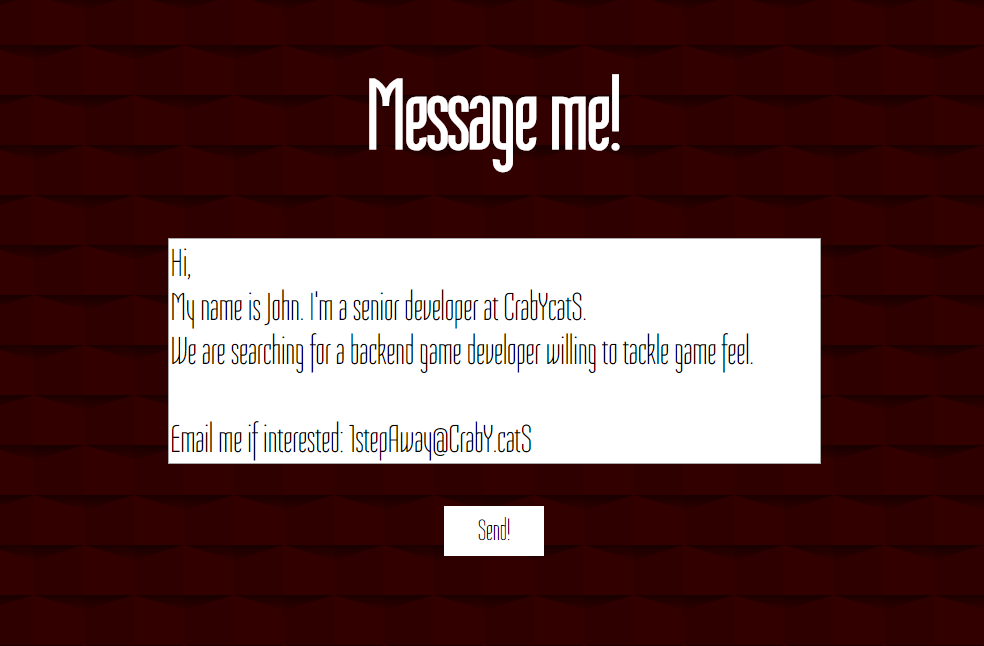
\includegraphics[width=14.6cm]{images/message.png}
				\caption{Izgled stranice za slanje poruke}
				\label{fig:message}
\end{figure}

Nakon što korisnik unese poruku i pritisne tipku send unesena poruka se prosljeđuje modelu u Java Spring MVC poretku te on popunjava mail i šalje poruku s gmail klijenta drugom gmail klijentu koji poruku smješta u pripadni sandučić.
Nakon obrade zahtjeva korisnik biva prebačen na poveznicu \textit{/sayHi/resultMessage} s pripadajućom porukom.
Najčešće "\textit{Mail successfully sent}" ili "\textit{Whoops, something went wrong, try again later}".

\section{Stranica s informacijama o programeru}
\qquad Stranica opisa programera nalazi se na poveznici \textit{mmedo.me/about}.
Slika 4.4 prikazuje gornji dio stranice opisa programera.

\begin{figure}[htb]
				\centering
				
\includegraphics[width=14.6cm]{images/about.png}
				\caption{Izgled stranice za prikaz opisa progamera}
				\label{fig:about}
\end{figure}

Na stranici su dostupne opće informacije o programeru, poput punog imena programera, njegove slike, razina obrazovanja, vještine programiranja koje programer posjeduje itd.
Na stranici se također nalazi brza poveznica na početnu stranicu.

\section{Dohvat životopisa programera}
\qquad Pri pokretanju programa, tijekom inicijalizacije kontrolera, kontroler iz memorije s diska učitava pdf datoteku životopisa u polje jedinice \textit{byte}.
Dohvat životopisa na stranici se vrši pritiskom na brzu poveznicu \textit{resume} na početnoj stranici.
Tada aplikacija prosljeđuje zahtjev drugom kontroleru na poveznicu \textit{mmedo.me/resume}. 
Kontroler učitano polje bajtova pohranjuje u http zaglavlje u kojem postavlja tip datoteke na pdf, te upute da datoteku web preglednik ne treba spremiti na disk, nego direktno prikazati u web pregledniku s ugrađenim pdf preglednikom.
Ako korišteni web preglednik nema ugrađen pdf preglednik datoteka će biti spremljena na disk.

\begin{figure}[htb]
				\centering
				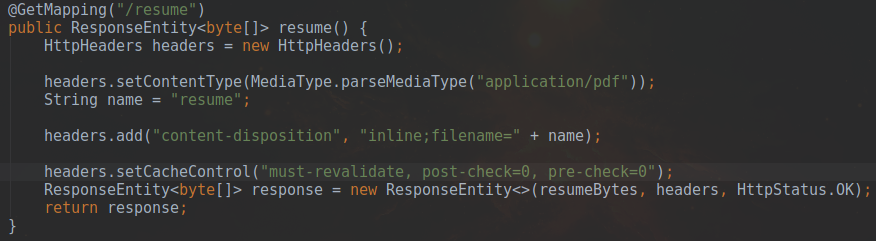
\includegraphics[width=14.6cm]{images/resume.png}
				\caption{Kod kojim se izvodi dohvat pdf datoteke}
				\label{fig:resume}
\end{figure}

\qquad Postupak je detaljno prikazan na slici 4.5.
Metoda \textit{resume()} u prvom retku stvara novo http zaglavlje.
U trećem retku metoda postavlja uputu web pregledniku kako da interpretira podatke koji će mu biti prosljeđeni (pdf format).
U šestom retku metoda daje uputu web pregledniku da pokuša otvoriti pdf datoteku s ugrađenim pdf preglednikom.
U sedmom retku metoda postavlja upute web pregledniku da ne koristi \textit{cache} memoriju za spremanje dokumenta, nego da ga svaki put ponovno dohvati.
Naposljetku, metoda stvara http odgovor i prosljeđuje ga web pregledniku.

\section{Stranica projekata}
\qquad Stranica projekata nalazi se na poveznici \textit{mmedo.me/projects}.
Stranicu projekata možemo zamisliti kao dvodimenzionalni koordinatni sustav.
Pomicanjem po ordinati koordinatnog sustava listamo projekte.
Pomicanjem po apscisi koordinatne mreže korisniku se prikazuju pojedinosti o odabranom projektu.
Takav pristup omogućen je korištenjem \textit{fullpage.js} biblioteke.
Ona nam omogućava sigurnost da klizačem ne možemo dospjet između dva polja u našoj koordinatnoj mreži.
Na slici 4.6 možemo vidjeti početnu stranicu projekata.

\begin{figure}[htb]
				\centering
				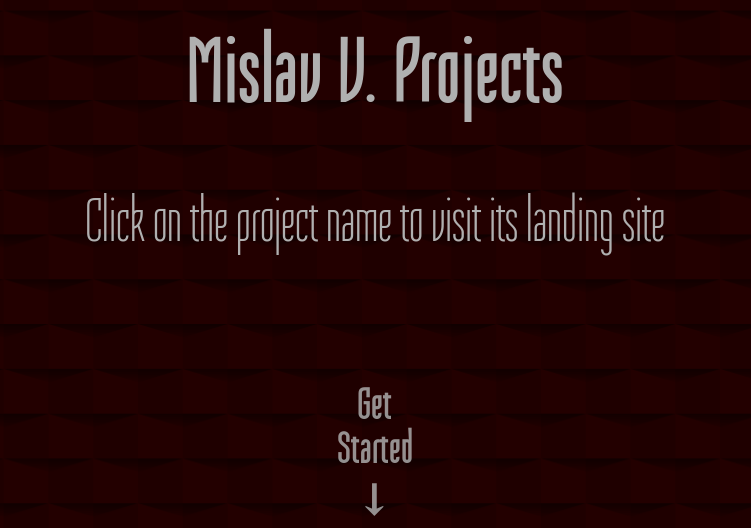
\includegraphics[width=14.6cm]{images/projects-main.png}
				\caption{Izgled početne stranice projekata}
				\label{fig:projects-main}
\end{figure}

Koristeći tipku klizača za pomicanje prema dolje na stranici dospjet ćemo na stranicu prikazanu slikom 4.7.

\pagebreak
Na slici možemo vidjeti naslov projekta te kratak opis projekta.
Pritiskom na naslov projekta web preglednik će biti preusmjeren na Git stranice projekta.
Također možemo vidjeti navigacijske tipke na lijevoj i desnoj strani u obliku trokuta.
Pritiskom na desnu tipku stranica koju trenutno gledamo pomaknuti će se ulijevo, te će novo polje koordinatne mreže doći u gledište.

\begin{figure}[htb]
				\centering
				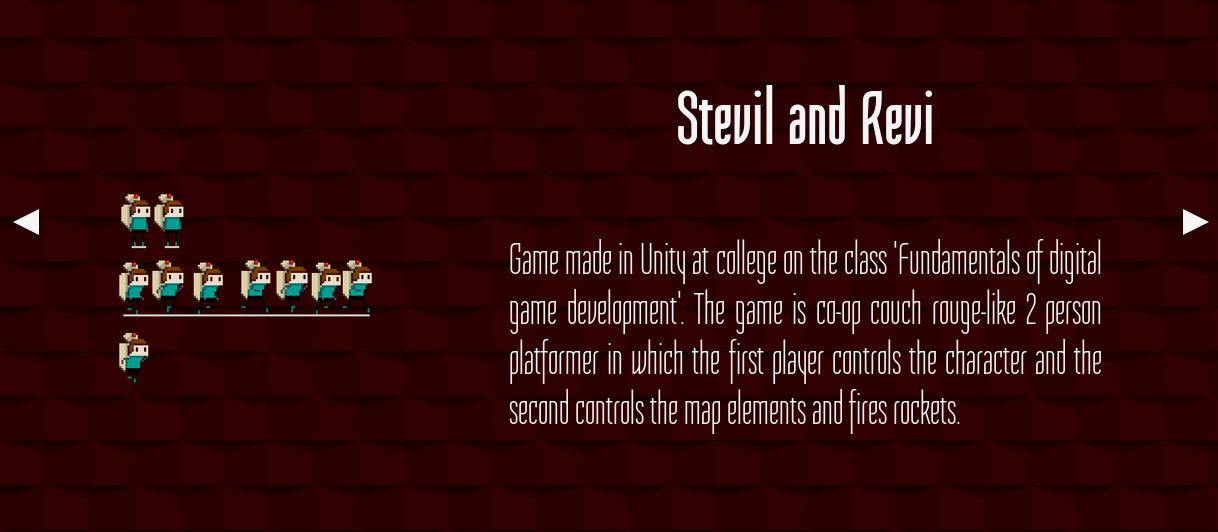
\includegraphics[width=14.6cm]{images/projects-img-text.png}
				\caption{Početna stranica konkretnog projekta}
				\label{fig:projects-img-text}
\end{figure}

Pritiskom desne tipke u obliku trokuta u gledište nam dolazi stranica prikazana slikom 4.8.
U konkretnom primjeru to je opis početka igre \textit{Stevil and Revi} koja je navedena kao prvi projekt na stranici projekata.

\begin{figure}[htb]
				\centering
				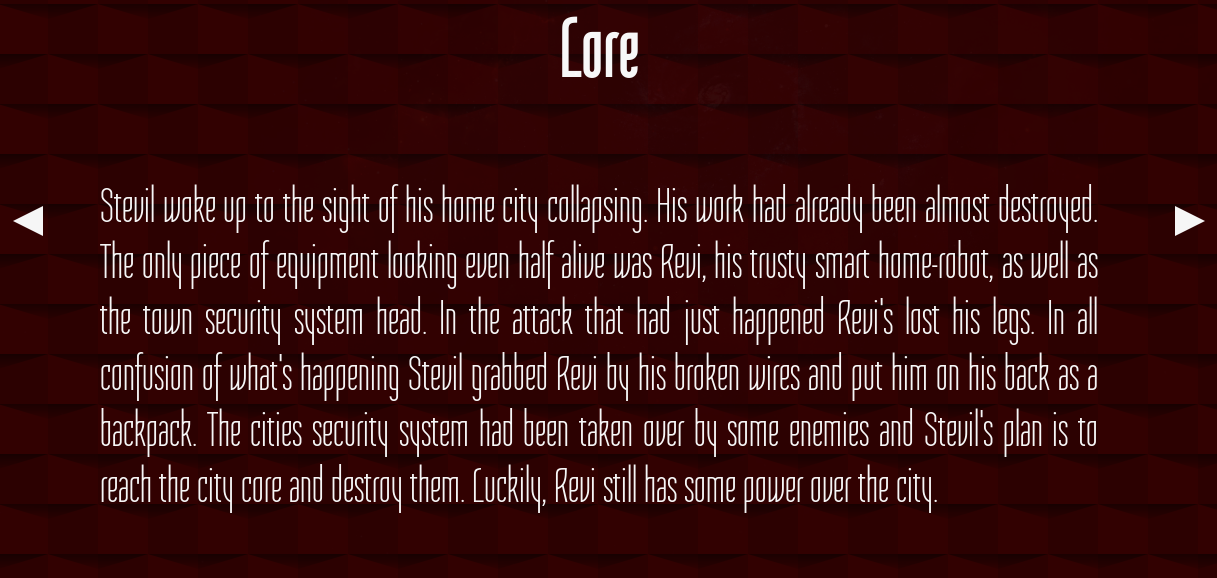
\includegraphics[width=14.6cm]{images/lore.png}
				\caption{Sekundarna stranica konkretnog projekta}
				\label{fig:lore}
\end{figure}

\section{Stranica pogreške}
\qquad Stranica pogreške nalazi se na poveznici \textit{mmedo.me/error}.
Svaki puta kada se dogodi pogreška korisnik je preusmjeren na tu stranicu.
To vrijedi i kada je unesena nepostojeća poveznica poput \textit{mmedo.me/invalid}.
Slika 4.9 prikazuje izgled stranice pogreške u slučaju upisa nepostojeće poveznice.

\begin{figure}[htb]
				\centering
				
\includegraphics[width=14.6cm]{images/error.png}
				\caption{Izgled stranice pogreške}
				\label{fig:error}
\end{figure}

\chapter{Zaključak}
\qquad Cilj ovog rada je napraviti vlastitu web aplikaciju za predstavljanje portfelja programera.
Cilj je uspješno postignut.
Razvijena stranica je dohvatljiva na adresi \textit{mmedo.me}.
Svi funkcionalni zahtjevi koje smo postavili su ispunjeni;
Opće i kontaktne informacije o programeru nalaze se na poveznici \textit{mmedo.me/about}.
Direktne poveznice na stranice Git repozitorija i stranice društvenih mreža nalaze se na početnoj stranici.
Razvijena stranica nudi mogućnost slanja poruke programeru bez unosa privatnih podataka, točnije email poruke.
Ta stranica se može dohvatiti na poveznici \textit{mmedo.me/sayHi}.
Odjeljak za projekte je uspješno realiziran na \textit{mmedo.me/projects}.
Naposljetku, životopis u pdf formatu je dostupan na poveznici \textit{mmedo.me/resume}.

\bibliography{literatura}
\bibliographystyle{fer}
\begin{thebibliography}{9}
\bibitem{programiranje-u-javi}
				Marko Čupić.
				\textit{Programiranje u Javi}.
				Inačica 30. rujna 2015.

\bibitem{awesome-portfolios}
				Awesome Creative Portfolio Websites,
				\\\texttt{github.com/iRaul/awesome-portfolios},
				\\\texttt{www.creative-portfolios.com}

\bibitem{java-spring}
				Spring by Pivotal,
				\\\texttt{spring.io}

\bibitem{w3schools}
				W3Schools Online Web Tutorials
				\\\texttt{https://www.w3schools.com/}

\bibitem{stackoverflow}
				StackOverflow,
				\\\texttt{https://stackoverflow.com/}

\bibitem{svgbackgrounds}
				SVGBackgrounds,
				\\\texttt{https://www.svgbackgrounds.com/}

\bibitem{three-image-transition}
				THREE Image Transition,\\
				\textit{Szenia Zadvornykh} \\
				\texttt{https://codepen.io/zadvorsky/pen/PNXbGo}
\end{thebibliography}

\begin{sazetak}
\qquad Prilikom traženja posla prednost je ako se programer može predstaviti potencijalnom poslodavcu sa svim projektima u kojima je sudjelovao i programskom podrškom koju je razvio.
Učinkovito predstavljanje može se postići uz pomoć jedne web stranice koja će omogućavati direktne poveznice na projekte do Git alata (sadržavati linkove na aktivne projekte) te omogućiti međusoban kontakt programera i poslodavca putem korisničkog sučelja.
Ovaj rad prikazuje realizaciju izrade jedne vlastite portfolio web stranice programera.

\kljucnerijeci{Java, Java Spring, Spring, MVC, portfolio, web, web stranica, portfelj, vlastita web stranica, web stranica programera, javascript}
\end{sazetak}

\engtitle{Software Developer Portfolio Web Application}
\begin{abstract}
\qquad When searching for a job it is an advantage if a developer can present himself to the potential employer with all projects he has worked on.
Many developers do this over Git websites, although not all projects one has worked on are available there.
That is why having a portfolio website where one can put links to every project is a big advantage.
Furthermore, a porfolio website is a great place to provide basic information or a form of contact.
This thesis covers creating a portfolio website with all the above mentioned features.

\keywords{Java, Java Spring, Spring, MVC, portfolio, web, website, site, developer website, javascript}
\end{abstract}
\end{document}
